\section{MPLS Signatures Validation}\label{validation}
% %%%%%%%%%%%%%%%%%%%%%%%%%%%%%%%%%%%%

%Figura u-turn
\begin{figure*}[!ht]
  \begin{center}
    \subfloat[Tunnel Length Distribution]{\label{hist_length}
      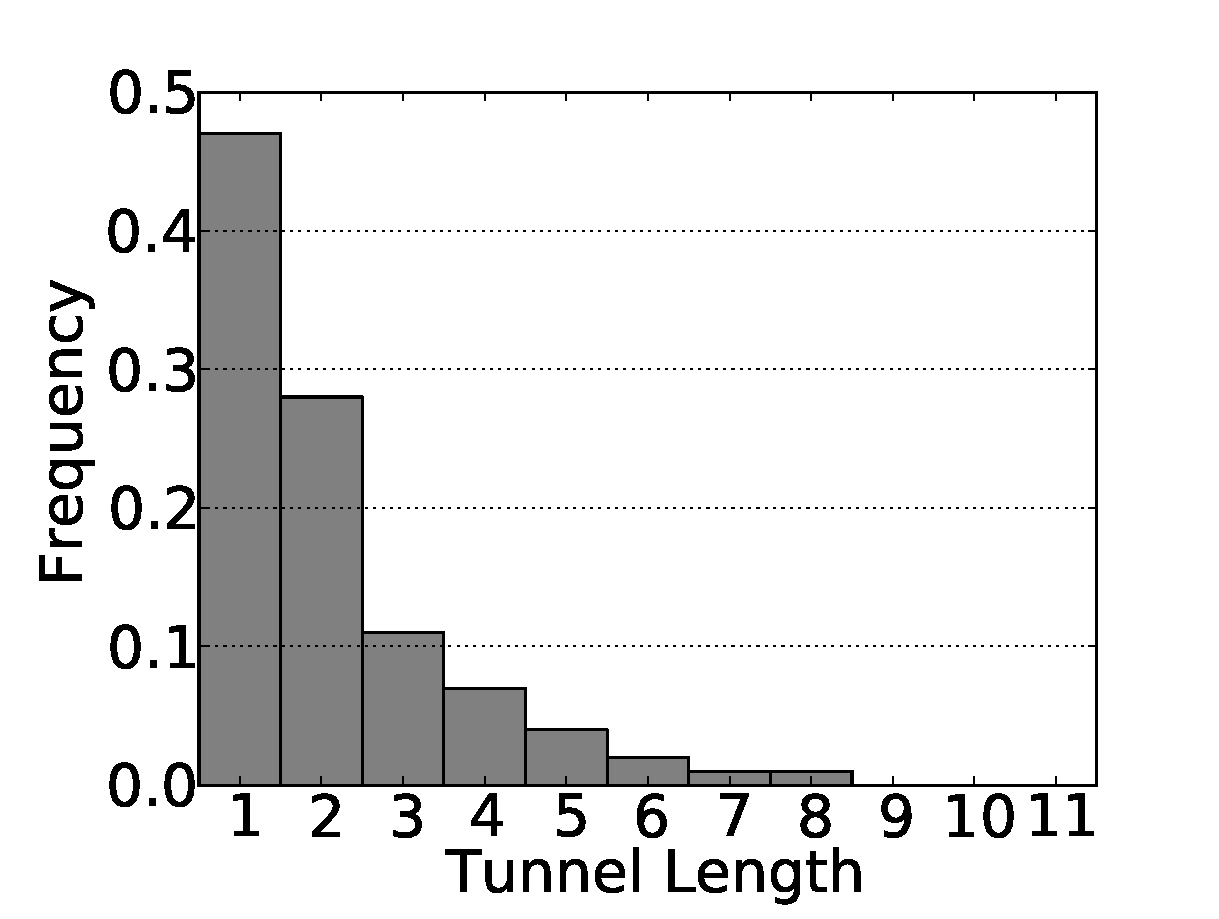
\includegraphics[width=6cm]{hist_length}}
      \hfil
    \subfloat[\textit{qTTL} and $n$-position comparison]{\label{n_vs_qttl}
      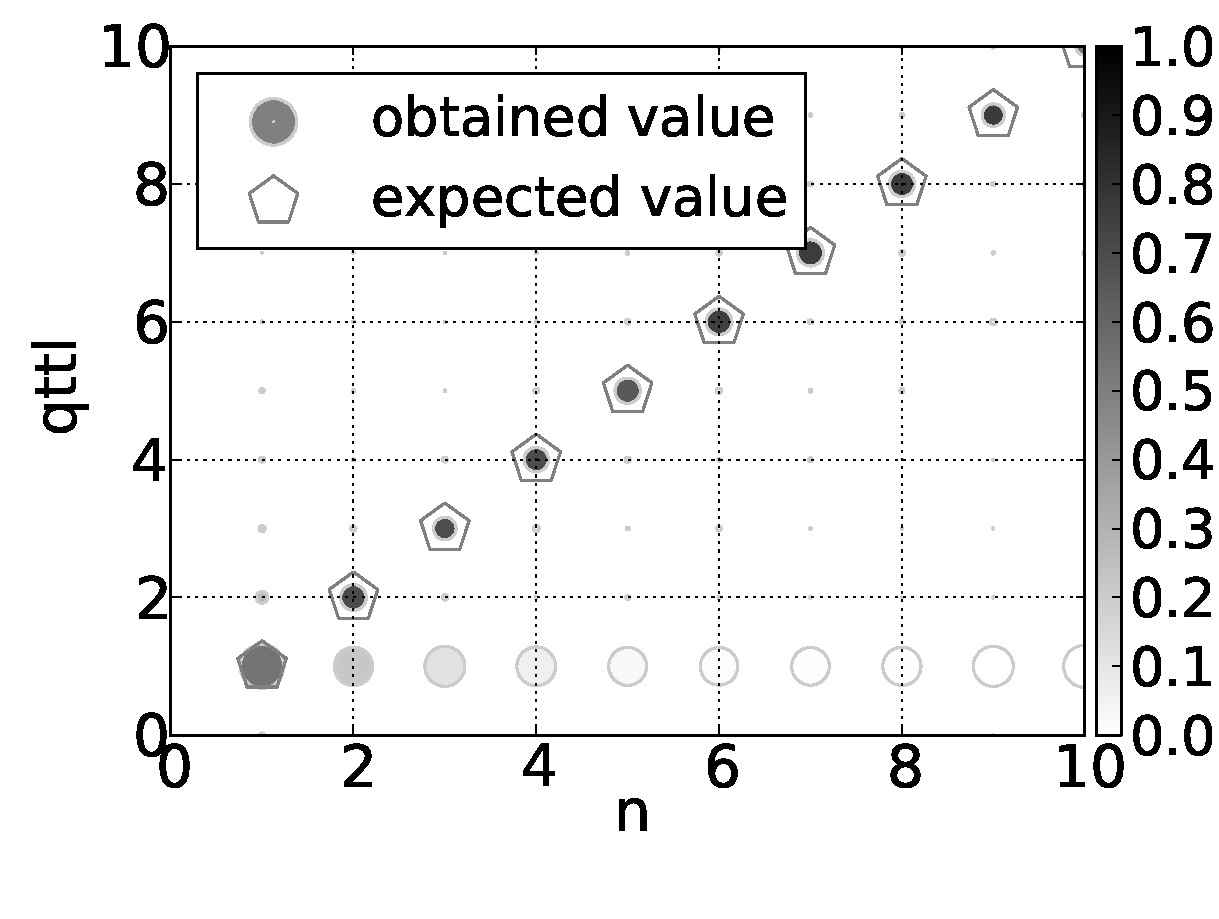
\includegraphics[width=6cm]{n_vs_qttl}} 
      \hfil
    \subfloat[\textit{u-turn} on LSRs where no other signature was found]{\label{fig_uturn_a}
      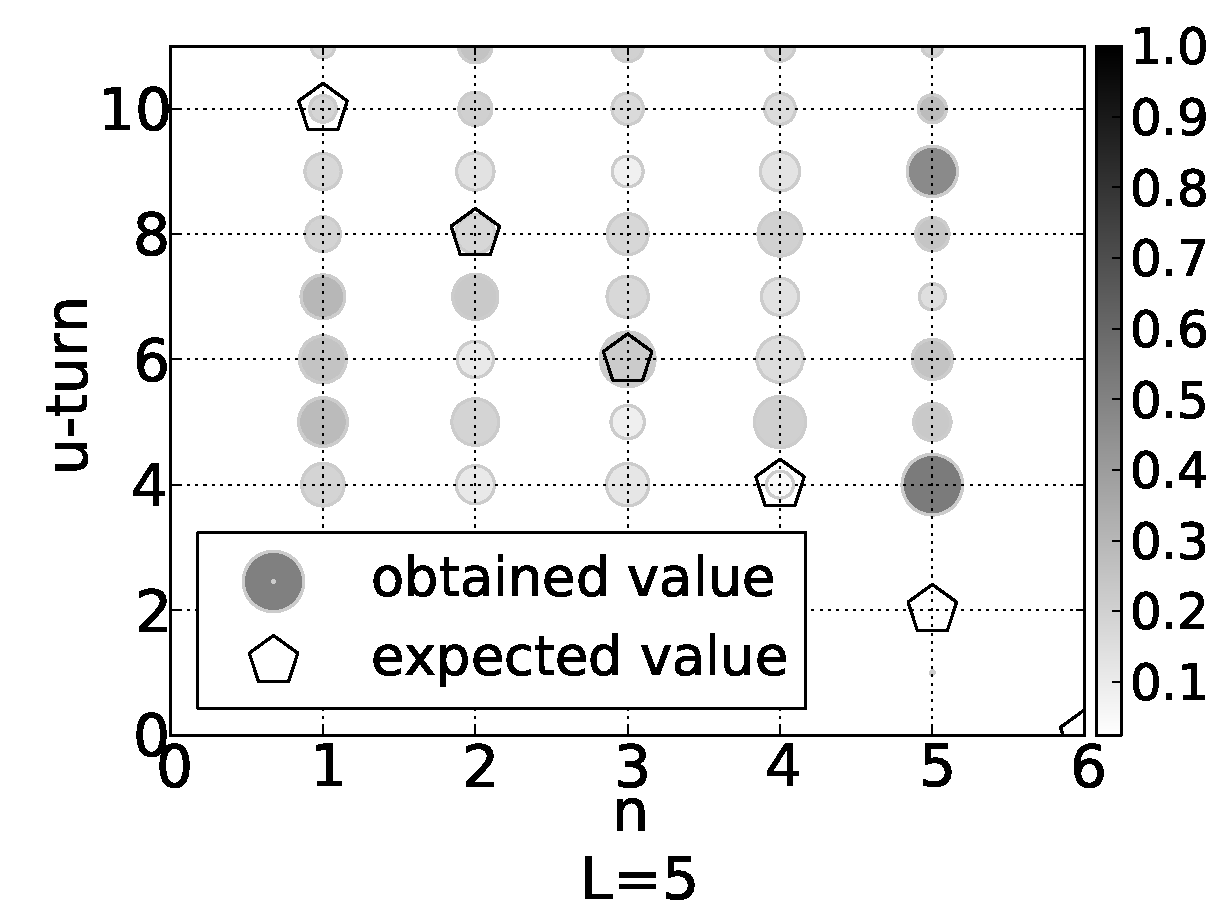
\includegraphics[width=6cm]{n_vs_uturn_L5}}
      \hfil
    \subfloat[\textit{u-turn} on LSRs revealed through RFC4950 and \textit{qTTL}]{\label{fig_uturn_b}
      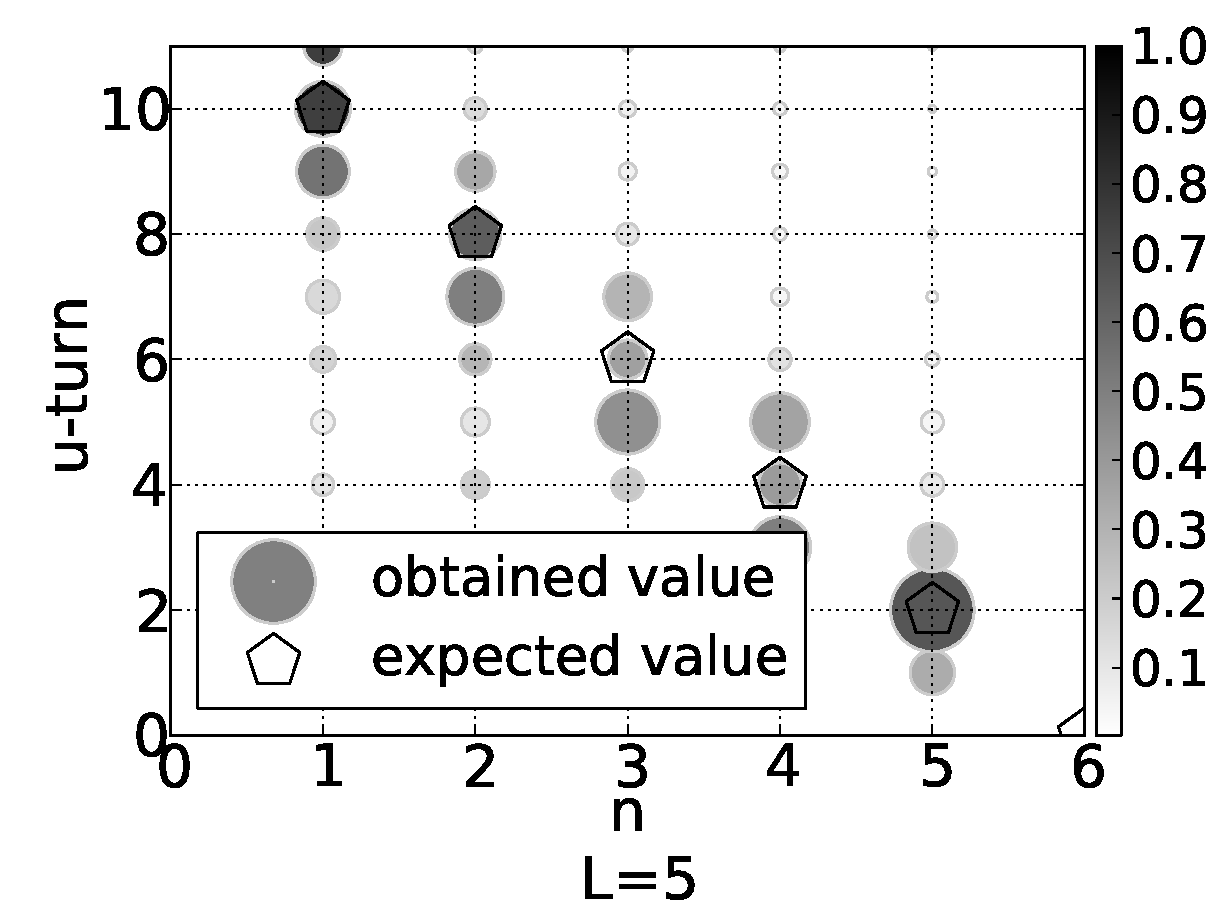
\includegraphics[width=6cm]{n_vs_uturn_L5_exp}}    
  \end{center}
  \caption{ Comparison between obtained and expected values for \textit{qTTL} and
  \textit{u-turn} signatures. On figures (b), (c) and (d) the circle size in the scatter plot is related with the occurrence frequency of \textit{y-axis} values regarding each $n$-position. The
  transparency of the circle is related with occurrence frequency of $n$-position  regarding each \textit{y-axis} value, e.g., on figure (b) for values where $n>1$, the biggest circles are mainly located on  $\textit{qTTL}=1$ and $\textit{qTTL}=n$ so this suggest that for a given $n$-position the \textit{qTTL} value usually takes either the value of $1$ or $n$; in the same way, the transparency value suggests that for a given \textit{qTTL} value the $n$-position usually takes the same \textit{qTTL} value. This suggest that \textit{qTTL} highly match with $n$-position.  \textbf{Figure (c)} and \textbf{Figure (d)} suggest that \textit{u-turn} value is overestimated. }
  \label{ig_signatures}
\end{figure*}

In this section we describe the used methodology to validate the MPLS signatures
revealed by traceroutes. As we described previously, the RFC9450 and
\textit{qTTL} signature are fingerprints that occurs just on MPLS behaviour,
while \textit{u-turn} could be related with issues not related with MPLS such as
load balancing. Thereby we mainly focus on test the \textit{u-turn} signatures.

If the RFC4950 is not implemented in the LSRs, the only way to reveal
an MPLS tunnel is trough \textit{qTTL} or \textit{u-turn} signatures. Both of
them are directly related with the position of MPLS within the tunnel:

\begin{itemize}
  \item[i] \textit{qTTL} value refers to the TTL of ICMP-\textit{echo}
  message when it enters to the MPLS  tunnel. A quoted TTL of $n$ in
  the incoming ICMP reply means that the sent probe
  expired $n$ hops later to ingress to the \textit{LSP}. In this way, we can say
  that a LSR that replies with $\textit{qTTL}=n$ appears  in the $n$ position of
  MPLS tunnel.
  \item[ii] The expected \textit{u-turn} value is related with the tunnel length and the position of the LSR within the tunnel (see section \ref{related.revealing})
\end{itemize}


%\begin{figure*}[!t]
%\centering
%\subfloat[Case I]{\includegraphics[width=2.5in]{box}%
%\label{fig_first_case}}
%\hfil
%\subfloat[Case II]{\includegraphics[width=2.5in]{box}%
%\label{fig_second_case}}
%\caption{Simulation results for the network.}
%\label{fig_sim}
%\end{figure*}

Our signature validation relays on the hypothesis that the MPLS position match
with the $n$-position  which an LSR is revealed by traceroute. Indeed,
we use a paris-traceroute \cite{BRICE06}  based tool in order to sure that the probes follow the
same path. In order to validate our hypotheses we first filter  tunnels revealed by \textit{u-turn} signature and we test our hypothesis on explicit tunnels and tunnels revealed by \textit{qTTL} signatures. Thereby we remove the bias caused by possible false
\textit{u-turn} signatures. The \textit{qTTL} values of our dataset  should to match with
$n$-position to validate our assumption, i.e., $\textit{qTTL}=n$.

The figure \ref{hist_length} shows the MPLS tunnel length distribution found in our dataset. Additionally,  we compare the \textit{qTTL} value and their respective $n$-position revealed by traceroute. The
results are showed in figure \ref{n_vs_qttl}. We noticed that \textit{qTTL}
signature highly match with the $n$-position, i.e., $q\textit{ttl}=n$.  A bias could
occur due to the limitation in our method to reveal the first LSRs in
the tunnel if it does not implement the RFC4950. %, i.e., the first LSR revealed by traceroute within the tunnel  ($n=1$) could correspond to a LSR with $\textit{qTTL}>n$. 
A second deviation
occurs due to possible load balancer presence in the follow path. In this case,
the traceroute probes follow paths with different lengths before to reach the
MPLS tunnel. This issue
produce that the same \textit{qTTL} value could be revealed many times in different
$n$-positions. The figure also shows that \textit{qTTL} 
takes frequently the value of $1$. This usually  means that \tpropagate is not implemented. However, we found that around $2\%$ of LSRs do not react to \textit{qTTL} signature, even if \tpropagate option is activated on the tunnel, i.e., some LSRs interfaces located at $i_{n-1}$  and $i_{n+1}$ tunnel positions have valid \textit{qTTL} signatures but the LSR interface located at $i_n$ position does not. We think that this issue occurs because some
routers update the IP-TTL to $1$ in the expired packet instead of keeping it
unchanged as usual. We found that in $58\%$ of the cases the $n$-position match with the
\textit{qTTL} value while in $36,3\%$ of cases the \textit{qTTL} signature is not
present and takes the value of $1$, and just $6,7\%$ of the cases presented
some bias around the expected value.

Once we proved  that \textit{qTTL} highly match with  $n$-position, we use
this position as a reference value to validate the \textit{u-turn} signature. In
this case, the expected value should to be $\text{u-turn}=2(L-(n-1))$ where $n$ is the
position of the LSR within the tunnel (particularity \textit{qTTL} value) and $L$ is the tunnel length. Because
\textit{u-turn} is commonly present in almost all LSRs, first we tested it in
MPLS tunnels  where other signatures were found, i.e., LSRs revealed
through RFC4950 and \textit{qTTL} signatures.
Secondly, we tested it on LSRs where \textit{u-turn} was the only
signature that allows us to reveal the MPLS tunnel. We use the filter ($\textit{u-turn}>3$) to
avoid false isolated \textit{u-turn} signatures. We compare the expected values and the
obtained values using a scatter plots in order to distinguish the amount of
signatures biased. The results for a given length are showed in figures
\ref{fig_uturn_a}, \ref{fig_uturn_b}. The same results were showed for other length values. Basically, we noticed that the obtained values are close to expected values either on LSRs revealed explicitly and through \textit{qTTL} signature (figure \ref{fig_uturn_a}). However on the set of  LSRs revealed just by \textit{u-turn} signatures (figure \ref{fig_uturn_b}) the values does not match. If we accept a bias of $ \pm 2$ around the expected value, we
noticed that on LSRs revealed through RFC4950 implementation and
\textit{qtll} signatures, the $60\%$ of obtained \textit{u-turn} values match
with the expected values. However, on LSRs
where no other signature was obtained (therefore where the \textit{u-turn} signature
is really useful), the obtained \textit{u-turn} signature just match in $25\%$. 
Therefore, we conclude that the LSRs revealed through \textit{u-turn}
signatures are highly overestimated. Mainly because MPLS tunnels are not the
only behaviour that could causes \textit{u-turn} signatures. Indeed, has been showed that load balancing is present in almost $39\%$ of traverse paths even between the same pairs source-destination \cite{BRICE07}. This issue is called \textit{per-flow} load balancing. Basically, packets that belongs to the same \textit{flow} are treated similarly \cite{BRICE06}. A \textit{flow} is identified by the first 32 bits of the IP \textit{payload}. In the case of ICMP messages, this fields refers to \textit{Type},
\textit{Code} and \textit{Checksum}. By definition, \textit{u-turn} signature is
based on two kinds of ICMP messages: ICMP \echoreply \textit{Code 11} and ICMP
\ttlexceeded \textit{Code 0}. Due to the different codes values
related with each ICMP message, there is no way to sure that they belong to the same \textit{flow} identifier and thereby to be sure that \textit{u-turn} value is caused just by MPLS tunnels.
